% Created 2022-03-22 Tue 23:18
% Intended LaTeX compiler: pdflatex
\documentclass[11pt]{article}
\usepackage[hidelinks]{hyperref}
\usepackage{amsmath}
\usepackage{amssymb}
\usepackage{amsfonts}
\author{Alexander Neville}
\date{\today}
\title{}
\hypersetup{
 pdfauthor={Alexander Neville},
 pdftitle={},
 pdfkeywords={},
 pdfsubject={},
 pdfcreator={Emacs 27.1 (Org mode 9.6)}, 
 pdflang={English}}
\begin{document}

\tableofcontents


\section{Data Structures}
\label{sec:orge14ce2b}

\emph{not implemented}

\section{Algorithms}
\label{sec:orgd53f464}

\emph{not implemented}

\section{Regular languages}
\label{sec:org8eaf998}

A \emph{regular language} can be defined by a regular expression or finite state machine.

\subsection{Mealy Machines}
\label{sec:orgf9cf509}

\emph{Mealy machines} are a type of FSM with an output determined by the current state and the input. The example in figure \ref{img:mealy}, is an exclusive OR operation on the last two inputs.

\begin{figure}[H]
\centering
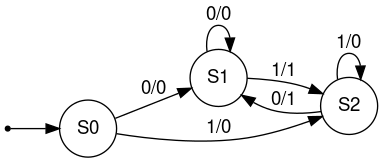
\includegraphics[width=0.4\textwidth, keepaspectratio, frame]{./images/mealy.png}
\caption{A typical Mealy machine}
\label{img:mealy}
\end{figure}

The state transition diagram can also be represented with a transition table.

\begin{center}
\begin{tabular}{rlrl}
\hline
Input & Current & Ouptut & Next\\
\hline
0 & S0 & 0 & S1\\
1 & S0 & 0 & S2\\
0 & S1 & 0 & S1\\
1 & S1 & 1 & S2\\
0 & S2 & 1 & S1\\
1 & S2 & 0 & S2\\
\hline
\end{tabular}
\end{center}

\subsection{Sets}
\label{sec:org011ea4f}

A set is an unordered collection of values, in which any one value may occur at most once. Sets may defined simply by listing each member.

\[A = \{2,4,6,8\}\]

There are a number of common sets:

\begin{itemize}
\item empty set: \(\{\}\) or \(\phi\), containing no elements
\item natural numbers: \(\mathbb{N} = \{1,2,3,4,5,...\}\)
\item whole numbers: \(\mathbb{Z} = \{...,-2,-1,0,1,2,...\}\)
\item rational numbers: \(\mathbb{Q}\), any value which can be expressed as a ratio
\item real numbers = \(\mathbb{R}\), the set of real world quantities
\end{itemize}

\subsubsection{Finite and Infinite Sets}
\label{sec:org8e7fdc9}

A finite set contains a number of elements which can be counted off to a particular number. Finite sets include \(\{1,6,8,9\}\) and \(\{1,3,5,...99\}\). The \emph{cardinality} of a set is the total number of elements in the set. Infinite sets may countable or not countable. Despite being infinite, \(\mathbb{N}\) is countable; it is possible to determine the next number in the set and count of elements. A fully countable set can be measured against a subset of the natural numbers, whereas a countably infinite set, can be countered interminably.

\subsubsection{Set Comprehensions}
\label{sec:orge571297}

More complicated sets may be defined by comprehension, a more compact syntax than writing out the whole set.

\[B = \{n^2 | n \in \mathbb{N} \wedge n < 5\}\]

\subsubsection{Cartesian Product of Two Sets}
\label{sec:org61e0201}

The \emph{Cartesian product} of two sets is written \(A \times B\) and is the set of all ordered pairs \((a, b)\) where \(a\) appears in \(A\) and \(b\) appears in \(B\). If \(A = \{2,4,6\}\) and \(B = \{1,3,5\}\), \(A \times B\) is:

\[\{(2,1), (2,3), (2,5), (4,1), (4,3), (4,5), (6,1), (6,3), (6,5)\}\]

\subsubsection{Sets and Subsets}
\label{sec:org85d99f6}

If every element in \(A\) is also a member of set \(B\), \(A\) is a subset of \(B\), written:

\[A \subseteq B\]

It could also be said that \(B\) is a superset of \(A\):

\[B \supseteq A\]

If \(B\) contains another element not in \(A\), then \(A\) is said to be a proper or strict subset of \(B\):

\[A \subset B\]

\subsubsection{Set Operations}
\label{sec:orgd9e072e}

The \emph{union} of \(A\) and \(B\) is all of the elements in either set or in both, written:


\[A {\displaystyle \cup } B\]

The \emph{intersection} of \(A\) and \(B\) is all of the elements both sets, written:

\[A {\displaystyle \cap } B\]

The difference between the sets \(A\) and \(B\) is all the elements in one set, but not the other, expressed:

\[A - B = \{x | x \in A \wedge x \not\in B\}\]
\end{document}
